%\documentclass[english,10pt]{beamer}
\documentclass[english, handout]{beamer}






 
%\usepackage{mathptmx}
%\renewcommand{\sfdefault}{lmss}
\usepackage[T1]{fontenc}
%\usepackage[latin9]{inputenc}
\usepackage[utf8]{inputenc}

\synctex=-1

\usefonttheme{professionalfonts}

%\setbeamertemplate{navigation symbols}{}
%\setbeamertemplate{caption}[numbered]


\useinnertheme{rectangles}
%http://tex.stackexchange.com/questions/11168/change-bullet-style-formatting-in-beamer

 \AtBeginDocument{
  \addtolength\abovedisplayskip{-0.4\baselineskip}%
  \addtolength\belowdisplayskip{-0.4\baselineskip}%
}%change the space between text lines and the math formula


\usepackage{pifont}
%Postscript ZipfDingbats font
%the command \ding{number}, will print the specified symbol

\usepackage{fontawesome}
%icon package
\DeclareFontFamily{U}{FontAwesomeOne}{}
\DeclareFontShape{U}{FontAwesomeOne}{m}{n}{<-> FontAwesome--fontawesomeone}{}
\DeclareRobustCommand\FAone{\fontencoding{U}\fontfamily{FontAwesomeOne}\fontseries{m}\fontshape{n}\selectfont}
\DeclareFontFamily{U}{FontAwesomeTwo}{}
\DeclareFontShape{U}{FontAwesomeTwo}{m}{n}{<-> FontAwesome--fontawesometwo}{}
\DeclareRobustCommand\FAtwo{\fontencoding{U}\fontfamily{FontAwesomeTwo}\fontseries{m}\fontshape{n}\selectfont}
\DeclareFontFamily{U}{FontAwesomeThree}{}
\DeclareFontShape{U}{FontAwesomeThree}{m}{n}{<-> FontAwesome--fontawesomethree}{}
\DeclareRobustCommand\FAthree{\fontencoding{U}\fontfamily{FontAwesomeThree}\fontseries{m}\fontshape{n}\selectfont}

%ftp://ftp.dante.de/tex-archive/fonts/fontawesome/doc/fontawesome.pdf
%http://tug.ctan.org/info/symbols/comprehensive/symbols-a4.pdf


\usepackage{amsmath,amssymb,amsfonts,bm,mathrsfs,mathtools}

\usepackage{tikzsymbols}
%\usepackage[tikz]{bclogo}



\usepackage{perpage}
\MakePerPage{footnote} %reset for each page
%\renewcommand{\thefootnote}{\fnsymbol{footnote}} %use symbol, limit less than 9 symbols



%%%% HIGHTLIGHT  and annotation &=%%%%%%%%
\usepackage{color,xcolor}
 \usepackage{todonotes}

\usepackage[normalem]{ulem}

\usepackage[many]{tcolorbox}

\tcbset{fonttitle=\scriptsize}
\tcbset{highlight math style={enhanced,
  colframe=red!40!black,colback=yellow!20!white,arc=2pt,boxrule=.2pt,
  }}
  \newtcbox{\otherbox}[1][]{nobeforeafter,math upper,tcbox raise base,
enhanced,frame hidden,boxrule=0pt,interior style={top color=green!10!white,
bottom color=green!10!white,middle color=green!50!yellow},
fuzzy halo=1pt with green,#1}
%%\tcbhighmath{math here}
%% \otherbox{math here}



%%%%% HIGHLIGHT %%%%%%
\newcommand{\hb}[1]{{\color{blue}{#1}}}
%\noindent\rule{\textwidth}{.5pt}

%:
\usepackage{soul}

\newcommand\hcancel[2][black]{\setbox0=\hbox{$#2$}%
\rlap{\raisebox{.45\ht0}{\textcolor{#1}{\rule{\wd0}{1pt}}}}#2}
%cross to delete

\newcommand{\mcb}[2]{\colorbox{#1}{$\displaystyle #2$}}
%highlight math

\newcommand{\hlfancy}[2]{\sethlcolor{#1}\hl{#2}}
%specified color , for\hl

\newcommand\myhl{\bgroup\markoverwith
  {\textcolor{yellow}{\rule[-.5ex]{2pt}{2.5ex}}}\ULon}



\mode<presentation>{ \usetheme{boxes} }

%write Matlab code
\usepackage{listings}
 \definecolor{dkgreen}{rgb}{0,0.6,0}
\definecolor{gray}{rgb}{0.5,0.5,0.5}
\definecolor{mauve}{rgb}{0.58,0,0.82}
\lstset{frame=tb,
  language=Matlab,
  aboveskip=3mm,
  belowskip=3mm,
  showstringspaces=false,
  columns=flexible,
  basicstyle={\small\ttfamily},
  numbers=none,
  numberstyle=\tiny\color{gray},
  keywordstyle=\color{blue},
  commentstyle=\color{dkgreen},
  stringstyle=\color{mauve},
  breaklines=true,
  breakatwhitespace=true
  tabsize=3
}

\usepackage[lastexercise]{exercise}

\newtheorem{ex}{Exercise}
\newtheorem{property}{Property}
\newtheorem{ag}{Algorithm}
\newtheorem{remark}{Remark}
\newtheorem{den}{definition}
\newtheorem{assumption}{Assumption}


\usepackage[nosolutionfiles]{answers}
\Newassociation{sol}{Solution}{ans}



\usepackage{empheq}
\usepackage{comment}
%\usepackage{lscape}
\usepackage{multirow}
\usepackage{url,hyperref}

\hypersetup{
 %   bookmarks=true,         % show bookmarks bar?
    unicode=false,          % non-Latin characters in Acrobat's bookmarks
    pdftoolbar=true,        % show Acrobat's toolbar?
    pdfmenubar=true,        % show Acrobat's menu?
    pdffitwindow=false,     % window fit to page when opened
    pdfstartview={FitH},    % fits the width of the page to the window
    pdftitle={My title},    % title
    pdfauthor={Author},     % author
    pdfsubject={Subject},   % subject of the document
    pdfcreator={Creator},   % creator of the document
    pdfproducer={Producer}, % producer of the document
    pdfkeywords={keyword1} {key2} {key3}, % list of keywords
    pdfnewwindow=true,      % links in new window
    colorlinks=true,       % false: boxed links; true: colored links
    linkcolor=red,          % color of internal links (change box color with linkbordercolor)
    citecolor=green,        % color of links to bibliography
    filecolor=magenta,      % color of file links
    urlcolor=cyan           % color of external links
}


\usepackage{subfigure,epsfig,graphicx,graphics}

\DeclareGraphicsRule{.tif}{png}{.png}{`convert #1 `dirname #1`/`basename #1 .tif`.png}
   \DeclareGraphicsExtensions{.pdf}




\newcommand{\hw}{ {\underline{\tt Homework }} }
\newcommand{\hws}{ {\underline{\tt Homework$\star$}} }
\newcommand{\optional}{ {\it optional} }

\newcommand{\MATLAB}{ \texttt{MATLAB}}
\newcommand{\python}{ \texttt{python}}
\newcommand{\Rlang}{ \texttt{R}}
\newcommand{\SAS}{ \texttt{SAS}}
\newcommand{\MC}{Markov Chain}


\newcommand{\tm}{transition matrix}
\newcommand{\rv}{random variable}
\newcommand{\spl} {supervised learning }
 

\newcommand{\dis}{\underline{\tt discussion}: }
\newcommand{\pri}{\underline{\tt principle}: }




\newcommand{\bq}{\scalebox{6}{\textbf{?} }}
\newcommand{\sq}{\scalebox{2}{\textbf{?} }}
\newcommand{\ck} {  {\scalebox{0.8} {\Interval}   } }

\newcommand{\eps}{\varepsilon}
\newcommand{\To}{\longrightarrow}

% 
\newcommand{\Dcal}{\mathtt{D}}
\newcommand{\Hcal}{\mathcal{H}}
\newcommand{\Ecal}{\mathcal{E}}
\newcommand{\Xcal}{\mathcal{X}}
\newcommand{\Ycal}{\mathcal{Y}}
\newcommand{\Zcal}{\mathcal{Z}}

%%Calculus 

\renewcommand{\d}{\ensuremath{\mathrm{d}}}
\newcommand{\dt}{ \ensuremath{\mathrm{d} t } }
\newcommand{\dx}{ \ensuremath{\mathrm{d} x} }
\newcommand{\dy}{ \ensuremath{\mathrm{d} y } }

%indicator function
\newcommand{\indf}{ \ensuremath{\mathbf{1} } }



%probability
\newcommand{\p}{ \mathbb{P}}
\newcommand{\prob}{{\Pr}}
\newcommand{\PP}{\mbox{PP}}%Poisson process
%condition prob
\newcommand{\cPr}[2]{{\Pr\left(#1\mid #2\right)}}

\newcommand{\FF}{{\mathbb{F}}}

\newcommand{\e}{ \operatorname{\mathbb E}}
\newcommand{\Var}{\operatorname{\mathbb{V} }}
\newcommand{\var}{\operatorname{\text{Var} }}
\newcommand{\MSE}{\operatorname{\text{MSE} }}

\newcommand{\Std}{\operatorname{std}}
\newcommand{\Cov}{\operatorname{cov}}

%Matrix  %mathbf
\newcommand{\Pb}{{\mathbf{P}}}
\newcommand{\Qb}{{\mathbf{Q}}}
\newcommand{\Mb}{{\mathbf{M}}}
\newcommand{\cb}{\mathbf{c}}
\newcommand{\bb}{{\mathbf{b}}}

\newcommand{\Tb}{\mathbf{T}}

\newcommand{\Wb}{\mathbf{W}}
\newcommand{\wb}{\mathbf{w}}
\newcommand{\Xb}{\mathbf{X}}

\newcommand{\xb}{\mathbf{x}}

\newcommand{\Wtn}{\mathbb{W}}
\newcommand{\btn}{\mathbf{b}}



\newcommand{\eye}{{\mathbf{I}}}
%identity matrix
\newcommand{\onem}{{\mathbb{1}}}
\newcommand{\idor}{\mathbf{1}}
\newcommand{\ii}{\mathbf{i}}
%imaginary symbol

\usepackage{tikz}

%State number
\newcommand{\snum}[1]{ \raisebox{.5pt}{\textcircled{\raisebox{-.9pt} {#1}}}}

 \usetikzlibrary{arrows}
\usetikzlibrary{shapes}

%\newcommand{\snum}[1]{%
 % \tikz[baseline=(char.base)]\node[anchor=south west, draw,rectangle, rounded corners, inner sep=1.4pt, minimum size=5mm,
   % text height=1.3mm](char){\ensuremath{#1}} ;}

\newcommand*\circled[1]{\tikz[baseline=(char.base)]{
            \node[shape=circle,draw,inner sep=.4pt] (char) {#1};}}


%real number
\newcommand{\Real}{{\mathbb{R}}}
%integer
\newcommand{\ZZ}{\mathbb{Z}}
%positive integer
\newcommand{\NN}{\mathbb{N}}



\newcommand{\inpd}[2]{\left\langle #1, #2 \right\rangle}
\newcommand{\abs}[1]{\left\vert#1\right\vert}
\newcommand{\norm}[1]{\left\|#1\right\|}
\newcommand{\wt}[1]{{\widetilde{#1}}}
\newcommand{\set}[1]{\left\{#1\right\}}
\newcommand{\partiald}[2]{  \frac{\partial #1 }{\partial #2}}



\newcommand{\ie}{{\it{i.e.}}}



\newcommand{\transpose}{\textsf{T}} % or, \intercal
\newcommand{\diag}{\textsf{diag}}
\newcommand{\tr}{{\textsf{T}}}
\newcommand{\rt}{{\textbf{r}}}

\DeclareMathOperator{\trace}{Trace}


\newcommand{\argmin}{ \operatornamewithlimits{argmin} }
\newcommand{\argmax}{ \operatornamewithlimits{argmax} }




\def\biz{\begin{itemize} }
\def\bizp{\begin{itemize}[<+->] }
\def\eiz{\end{itemize}}


\def\bfm{\begin{frame}}
\def\efm{\end{frame}}

\def\bena{\begin{enumerate}[<+-| alert@+>]}
\def\ben{\begin{enumerate}}
\def\een{\end{enumerate}}


\def\bbk{\begin{block} }
\def\ebk{\end{block}}






\makeatletter
%%%%%%%%%%%%%%%%%%%%%%%%%%%%%% Textclass specific LaTeX commands.
 % this default might be overridden by plain title style

%%%%%%%%%%%%%%%%%%%%%%%%%%%%%% User specified LaTeX commands.
%\usetheme{Warsaw}
\usetheme{Boadilla}
% or ...



%\setbeamertemplate{footline}[text line]{} % makes the footer EMPTY
%\setbeamertemplate{footline}[page number]{} % makes the footer EMPTY

%\usecolortheme{orchid} %not use is better 

\setbeamertemplate{footline}[text line]{%
  \parbox{\linewidth}{\vspace*{-2pt}Xiang Zhou\hfill CityU\hfill \insertpagenumber}}
%\setbeamertemplate{navigation symbols}{}

%\setbeamercovered{transparent}
% or whatever (possibly just delete it)


%\usepackage{babel}
\makeatother



 %
%\addtobeamertemplate{frametitle}{}{%
%\begin{tikzpicture}[remember picture,overlay]
%\node[anchor=south east,yshift=2pt] at (current page.south east) {
\includegraphics[height=0.6cm]{CityU_Logo_Basic_Signature.eps}};
%\end{tikzpicture}}
%

\beamerdefaultoverlayspecification{<+->}
%the presentation acts as though a \pause command has been inserted between every two bullets, without the actual need to write \pause after each item.



\title{Classification: Support Vector Machine}
\author{
\includegraphics[height=1.1cm,width=2.2cm]{../CityU_Logo_Basic_Signature.eps}
\\ $\ $ \\
Xiang Zhou  \\ $\ $ \\
}
\institute[]{  School of Data Science 
\\
 Department of Mathematics
\\
City University of Hong Kong
\\
~~
\\
\textup{  }
}

\date[]{}



\begin{document}
 
 


\maketitle
 
 
 
\frame{{SVM: support vector machine}
Mainly developed and was dominantly hot in computer science / pattern recognition  

\biz
\item Vapnik 1995:  Geometric Viewpoint + Primal-Dual for Quadratic Programming (+ Kernel trick, new def of metric)   ~~
\item Major developments throughout
1990’s
\item Has good generalization properties;
\item One of the most important and successful 
developments before deep learning. 
\eiz


\begin{table}
\begin{center}
\begin{tabular}{c|c}
Method & main properties
\\
\hline
\hline
\hb{maximal margin classifier}
 & only for linear separable dataset
  \\
\hline
  \hb{support vector classifier}
  & slack variable, linear classifier 
 \\
 \hline
  \hb{support vector machine} & kernel trick, nonlinear classifier
  \\ \hline
\end{tabular}
\end{center}
\caption{Development of SVM}
\end{table}

\footnote{ Sollich 2002: \href{https://link.springer.com/content/pdf/10.1023/A:1012489924661.pdf}{Bayesian Viewpoint} of SVM }

\footnote
{
We do not  discuss here the numerical optimization   part of SVM 
(\href{http:/uito/www.robots.ox.ac.uk/~az/lectures/ml/index.html}{ref}).
The focus here is the geometric intuition and modelling.
}

}
\frame{{Linear Separation  for binary classification}
Binary classification problem:  dataset $\set{x_i, y_i}$ where $y_i\in \mathcal{Y}=\set{-1,1}$.
\biz
\item Logistic regression assumes: log odd $\log h(x)$ is linear in $x$. 
The decision boudary
$h(x)=0.5$ is equivalent to $\beta \cdot x   =0.5$ 
\item The LDA's  the discriminant function $\delta(x)$ is also linear in $x$.
\item SVM is also a linear classifier, with a strong geometric intuition.
\eiz

Summary:
  \biz
 \item 
The logistic  regression =
sigmoid  activation function 
+ 
linear feature assumption 
+ maximum likelihood
\item 
The  linear discriminant analysis (LDA) =
Bayes classifier +  Gaussian mixture +
equal variance   assumption  
\item 
The support vector machine (SVM) = 
linear classifier 
+ max margin
\eiz

}

\frame{Note the notations different from logistic regressions:
\biz
\item $\mathcal{Y} =\set{-1,1}$, not $\set{0,1}$
\item the discriminant function is generally denoted by $f$.
The classifier  $\phi(x) := \mbox{sign} f(x)\in \set{-1,1}$.
Then decision boundary is $f(x)=0$, not $h(x)=0.5$.
\eiz
This set of notation is convenient because
if $y $ belong to $ \set{-1,1}$
$$\tcbhighmath
{\mbox{sign} f(x) = y \iff  y f(x)  >0.}$$ 

 Note
  $\mbox{sign} f(x)  = \mbox{sign}( \lambda f(x) )$ for any $\lambda>0$. 
 }
 
\frame{

\begin{ex}
 A linear discriminant function is $f(x)=w\cdot x + b$.
Assume $\norm{w}=1$.
Given a point $x^*$, show the  signed distance between $x^*$
and the hyperplane $f(x)=0$ is $$ {f(x^*)}$$ ( or $f(x^*)/\norm{w}$ in general).
The positive sign of $f(x^*)$ means that $x^*$ on the same side of the hyperplane as the normal direction vector $w$.
\end{ex}

Given one data example $(x_i, y_i)$,
if $f$ correctly classifies $x_i$, then $\mbox{sign} f(x_i)=y_i$,
the absolute  distance to the hyperplane $f(x)=0$ is 
$$\frac{1}{\norm{w}}\abs{f(x_i)} = \frac{1}{\norm{w}} f(x_i) \cdot \mbox{sign} f(x_i) = 
\tcbhighmath{
 \frac{1}{\norm{w}} {f(x_i) y_i }=:M_i},$$
which is   the {\bf  margin} of $x_i$ and $y_i$  to the separating hyperplane.
If $f$ misclassifies $x_i$, then $M_i <0$.
}

\frame{
 
\begin{definition}[margin]
Given   the dataset $(x_i, y_i), i=1,\ldots, n$  
and a linear function $f(x)=w\cdot x+b$, then 
the margin
\footnote{
Sometimes, the margin refers to $2M$, the distance between 
the two hyperplanes 
$w\cdot x + b = \pm M/\norm{w}$.
}
 of the dataset $(x_i, y_i), i=1,\ldots, n$ to the hyperplane $f(x)=0$ is 
\[
M= \min_{1\leq i \leq n} M_i =\min_{i} \set{ y_i (w\cdot x_i +b) / \norm{w} }
\]
The {\bf support vectors} are the collection of $\set{x_j}$
such that $M=y_j (w\cdot x_j +b)$.
\end{definition}
}

\frame{

\biz

\item $M$ depends on $w, b$ and the dataset $\set{x_i,y_i}$.
\item If there exists a linear function $f=w\cdot x+b$ such that 
$M>0 \iff $ the dataset is linearly separable, i.e. 
$$\mbox{sign}f(x_i) = y_i, \forall i.$$

\item
The margin $M$ is a function of $w$ and $b$,
we consider its maximal value over the choice of $w$ and $b$:
\begin{equation}\label{maxm7}
M^*:=\max_{w,b} M(w,b)=\max_{w,b}  \left(  \min_{i} \set{ y_i (w\cdot x_i +b) / \norm{w} }
\right)
\end{equation}
\item  If $M^*$ is positive, then the corresponding optimal $w^*$ and $b^*$ :
 the dataset is linearly separabble
\item If $M^*$ is negative,  then for any $w$ and $b$, $M<0$,
i.e., there exist some data $i$ such that $M_i<0$, misclassified.
The dataset is not linearly separable.

\eiz
}

\frame{{Maximal Margin Classifier}
Write \eqref{maxm7} in standard constrained optimisation form: 
\begin{definition}[maximal margin classifier]
{The maximal margin classifier} solves the problem 
\begin{equation}\label{eq:mmc}
\begin{split}
&\max_{w\in \Real^d,b\in \Real} M
\\
\mbox{subject to} ~&~~
\norm{ w} =1\\
&  y_i (w\cdot x_i +b) \geq M , \forall i
\end{split}
\end{equation}
\end{definition}
\biz
\item 
The equivalent form of maximal margin classifier is
\begin{equation}\label{eq:mmc2}
\begin{split}
&\max_{w\in \Real^d,b\in \Real} M
\\
\mbox{subject to} ~~
 &  y_i (w\cdot x_i +b) / \norm{w}\geq M , ~~  i=1,2,\ldots, n
\end{split}\end{equation}
\item The constraint $\norm{w}=1$ is only for the uniqueness of $w$ and $b$;
without this constraint, the solution  is a family of the linear discriminant functions
$\set{\lambda f^{*}(x): \lambda>0}$, which all share 
the {\bf same} classifier $\phi^{*}=\mbox{sign}f^*$.

\eiz

}

\frame{
\begin{ex}[XOR]
Suppose the dataset has $n=4$ examples in $\Real^2$ plane as follows:
\begin{tabular}{ll}
$ x_1$=(1, -1)&  $y_1$ = -1\\
 $x_2$=(1, 1) &  $y_2$ =   1\\
 $x_3$=(-1, 1)&  $y_3$ = -1\\
 $x_4$=(-1, -1)&  $y_4$ = 1
\end{tabular}.
Find the maximal margin classifier $f(x)=w_1 x_{(1)} + w_2 x_{(2)} + b$
where $x=(x_{(1)},x_{(2)})\in\Real^2$
\end{ex}
{\tiny
\begin{align*}
&\max_{w\in \Real^d,b\in \Real} M
\\
\mbox{subject to} ~&~~
w_1^2 + w_2^2 =1\\
&  w_1 + w_2 + b \geq M  
\\
&  -w_1 - w_2 + b \geq M  
\\&
  w_1 - w_2 - b \geq M  
  \\&
    -w_1 + w_2 - b \geq M  
\end{align*} 
The constraints are equivalent to $\abs{w_1+w_2}\leq -M+b$ and $\abs{w_1-w_2}\leq -M-b$.
Then $\abs{w_1}\leq -M$. So any admissible $M$ is negative.
It is easy to show that 
$M\pm b\leq 0$. So the possible max of $M$ is $M=b$ or $M=-b$.
If $M=b$, then $w_1=-w_2=\pm b$ and $f(x)=(-x_1+x_2\pm1)/\sqrt{2}$.
If $M=-b$, then $w_1=w_2=\pm b$ and the solution is 
$f(x)=(-x_1-x_2\pm1)/\sqrt{2}$
}

}

\frame{{Cover theorem: increasing dimension improves linear separability}

\href{http://web.mit.edu/course/other/i2course/www/vision_and_learning/perceptron_notes.pdf}
{Cover’s theorem}:
\begin{quote}
“pattern-classification problem cast in a high dimensional
space non-linearly is more likely to be linearly separable
than in a low-dimensional space”
\end{quote}
Kernel trick: 
\begin{center}
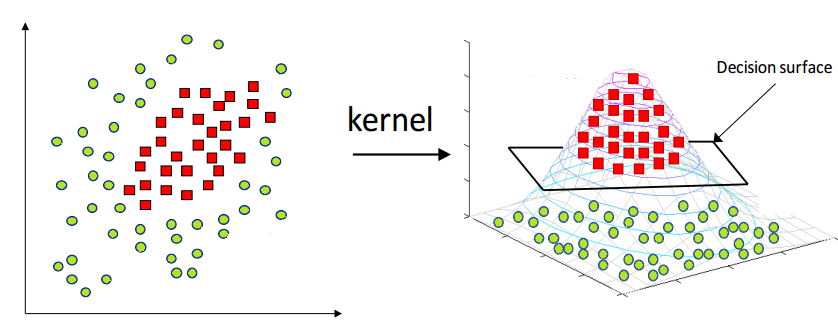
\includegraphics[width=0.6\textwidth]{kernel-trick.png}
\end{center}
 \href{https://www.hackerearth.com/blog/machine-learning/simple-tutorial-svm-parameter-tuning-python-r/}{image source}

}


\frame{
Recall the maximal margin classifier \eqref{eq:mmc2}
Since we can scale $w,b$ by a {\bf positive} factor arbitrarily, we
can assume  $M>0$ and use the normalization $ M \norm{w} =1 $ {\it if the dataset is linearly separable},
instead of using the normalization $\norm{w}=1$.
Then
\begin{equation}\label{eq:mmc3}
\begin{split}
&\min_{w\in \Real^d,b\in \Real} \frac12 \norm{w}^2
\\
\mbox{subject to} ~~
 & \tcbhighmath{ y_i (w\cdot x_i +b) \geq 1 , \forall i}
\end{split}
\end{equation}
\biz
\item
Now there is NO admissible solution if the dataset is  not linearly separable, in contrast to  \eqref{eq:mmc2} and \eqref{eq:mmc}.
\item The problem  \eqref{eq:mmc3} is the standard quadratic programming problem \faSmileO .
\item
The margin now is $M=\frac{1}{\norm{w}}$.
 
\item The support vectors are those on the two hyperplanes 
\[ \boxed{ w\cdot x + b =\pm 1},\]
i.e., the inequality constraints at these support vectors 
actually are equalities.

\par 
\eiz

}


\frame{{\faLightbulbO
~Support Vector Classifier}
\framesubtitle
{soft margin and slack variable for nonseparable dataset}

\underline{But linear separation assumption is too strong in practice}

The non-separable case means there are some examples $(x_m, y_m)$ such that
$y_m (w\cdot x_m +b) < 0$.  Then by adding $n$ slack variables $\xi=(\xi_1,\ldots, \xi_n)$, we have the support vector classifier 
\begin{definition}[support vector classifier]
\begin{align}
&\min_{w\in \Real^d,b\in \Real, \xi \in \Real^n} \frac12 \norm{w}^2
\\
\mbox{subject to} ~~
 &  y_i (w\cdot x_i +b) \geq 1-\xi_i , \forall i
 \\
 &\xi_i \geq 0, \forall i
 \\
 & \sum_{i=1}^n {\xi_i} \leq s
\end{align}
where the constant $s>0$ is a tuning parameter.
\end{definition}
This is in the standard form of 	quadratic programming. 
}
\frame{{Remarks on relaxation budget}

\biz
\item hyperparameter $s$ controls the budget of relaxation:
\biz
\item $s=0\iff \xi_i \equiv 0$,   maximal margin classifier becomes \eqref{eq:mmc3}(for linearly separable case)
and  does not allow violation of the margin.
\item 
If $s=+\infty$, any $w$ and $b$ are admissible, and then the optimal  $w^*=0$, $b$ arbitrary:
huge bias, low variance 
\eiz
\item The budget $\sum_i \xi_i < s$ can be rewritten as the penalty form 
with the parameter $C>0$
\begin{align}
\label{eq:svc9}
&\min_{w\in \Real^d,b\in \Real, \xi\in\Real^n} \frac12 \norm{w}^2
+  C \sum_{i=1}^n {\xi_i}
\\
\mbox{subject to} ~~
 &  y_i (w\cdot x_i +b) \geq 1-\xi_i , \forall i
 \\
 &\xi_i \geq 0, \forall i
 \end{align}
 Totally, $d+1+n$ unknowns.
\eiz}

\frame {{Interpretation of slack variables at optimality }
There are two constraints:
\[  y_i (w\cdot x_i +b) \geq 1-\xi_i , ~\mbox{ and } \xi_i \geq 0\]
At the optimal values, some constraints may be active, some others may be inactive.

With the abuse of language, we define ``margin''
as the set between two hyperplanes 
$
\mathcal{M}:=\set{x:    \abs{w\cdot x + b}  \leq  1}
$
\biz
\item $\xi_i = 0$, then   $x_i$ is correctly classified and even better that it is not inside of the margin $\mathcal{M}$.
Furthermore, if additionally  $y_i (w\cdot x_i +b)  = 1$, then $x_i$ is a support vector, sitting on the boundary of margin.
\item $\xi_i >0$,  then  $y_i (w\cdot x_i +b) = 1-\xi_i$ and is less than $1$,
  $x_i$ violates the margin boundary and enters $\mathcal{M}$;
\biz
\item  $0<\xi<1 $:  $x_i$ is still correctly classified but too close to the decision boundary. 
\item $\xi_i >1$ :   $y_i (w\cdot x_i +b)$ is negative so,       $x_i$ is misclassified.
\eiz
\eiz

\footnote{The theory of constrained optimization such as linear programming theory is helpful in understanding this part.}
}

 
\frame{


\begin{center}
\begin{figure}
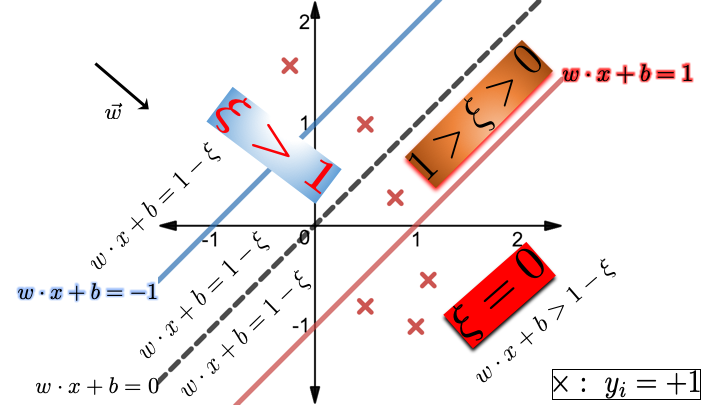
\includegraphics[width=0.8\textwidth]
{SVM-slack.png}
\caption{The slack variables for the data point  in class $+1$, markers(``$\times$'').
$x\in \Real^2$.}
 \end{figure}
 \end{center}
 The larger value of $\xi_i$, the further the point $x_i$ away from the correct domain.
This justifies the penalty of $\sum_i \xi_i$.
}


\frame{
\begin{center}
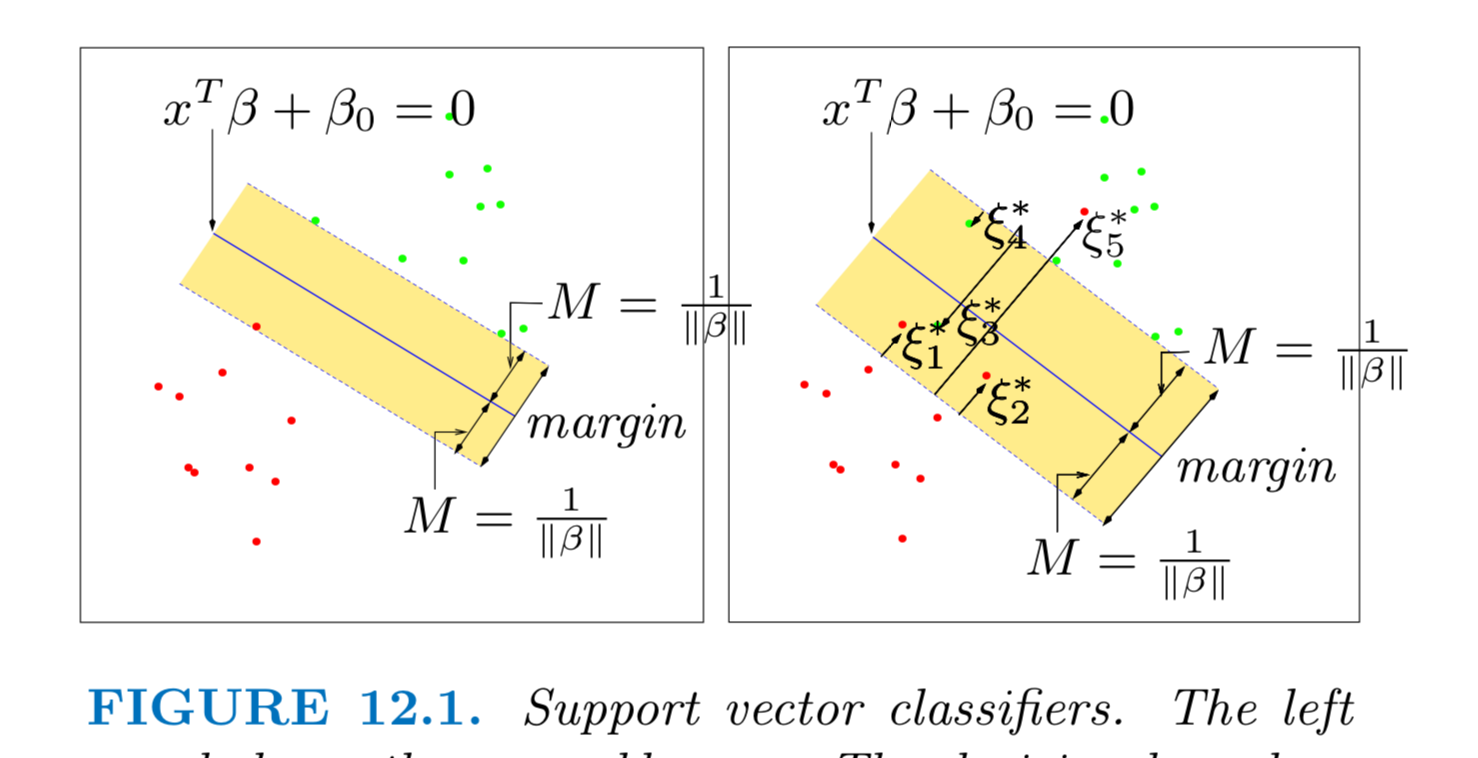
\includegraphics[width=0.98\textwidth]
{SVC-margin-slack.png}
\par From [ESL]: here $\xi^*_i: =M \xi_i$
\end{center}
Exercise:   discuss the range of $\xi^*_i=M \xi_i$ in the right figure.
}


\frame{{Interpretation  of Support vectors}
The support vectors are those $x_i$ such that 
$y_i (w \cdot x_i +b ) = 1-\xi_i$.
This equation of $w$, $b$ can  easily solved if 
 these support vectors as well as $\xi_i$ are known. 
In fact 
the solution of SVC is 
\[
w^* = \sum_{ i \in S }\hat{\alpha} y_i x_i
\]
where $S=\set{i: y_i (w \cdot x_i +b ) = 1-\xi_i}$.
Refer to Section 12.2.1 in [ESL].

 \biz
 \item 
Complexity of the classifier is characterized by the number
of support vectors rather than the dimensionality.
   \item The solution is insensitive to the outliers  (the data points significantly far away from the decision boundary).
   \eiz
}



%%%--------------------------------------------------------------------

\frame {

\frametitle{  SVM with kernel tricks: nonlinear decision boundaries}

The key idea of extending linear SVC, and many other linear procedures, to nonlinear is to:
\begin{itemize}
\item Enlarge the predictor space using basis expansion functions $h_1(x),\ldots,h_M(x)$
\item Construct a linear separating hyperplane $f(x) =  w\cdot h(x) + b$ in the enlarged space for better training performance
\item The linear separating hyperplane in the enlarged space can be translated into a nonlinear separating hyperplane in the original space.
\end{itemize}

The procedure is to replace $x$ in SVC by $h(x)$ in SVM.
We do not discuss the details further: this is a general principle.
}



\frame{
NEXT:

Rewrite the Constraint Optimization  form of SVC 
into the classic form 

{Loss function  + Penalty }


\bigskip

Note that two constraints in SVC 
$ y_i f(  x_i  ) \geq 1-\xi_i  $  and $\xi_i \geq 0$ together 
are equivalent to 

$$\xi_i \geq \max\set{0, 1-y_if(x_i)}=: (1-y_i f(x_i))_+.$$


}


\frame{{   SVM= hinge Loss + $L_2$-Regularization}

Then the SVC  in \eqref{eq:svc9}
is equivalent to 
\begin{align*}
&\min_{w\in \Real^d,b\in \Real, \xi \in \Real^n} \frac{1}{2} \norm{w}^2 + C\sum_{i} \xi_i
\\
\mbox{subject to} ~~
  &\xi_i \geq (1-y_i (w\cdot x_i + b))_+, \forall i
 \end{align*}
 which is equivalent to
 \begin{equation}
\min_{w\in \Real^d,b\in \Real} \frac{1}{2C} \norm{w}^2 + \sum_{i} (1-y_i (w\cdot x_i + b))_+
 \end{equation}
 This is the form of  (hinge) loss + ($L_2$) regularization
\[
\otherbox{
\ell_{ {hinge}}(y,f) = (1-y f)_+ , ~~ y\in \set{-1,1}, f \in \Real}
\]
}


\frame{
The population risk is 
\[
 \Ecal ( f) =  \e \ell_{ {hinge}} (Y, f(X))
\]
The penalty for the roughness of $f$ :
$R(f)=\norm{f}$.

When  $f(x)=w\cdot x +b$, 
\begin{equation}
\min_{w,b} \sum_{i=1}^n  \ell_{ {hinge}}(y_i, f(x_i)) + \frac{\lambda}{2}\norm{w}^2
\end{equation}

\biz
\item
$\lambda = 1/C$: the budget for relaxation.
\item $\lambda>0$: the penalty on the margin-relevant variable $\|w\|$.
\item The soft margin  performs like regularization; so the SVM is usually 
good at generalization.
\eiz
}

\frame{
 {\bf logistic regression :  binomial deviance Loss without  Regularization}

Recall the logistic regression solves
\begin{equation}
\min_{f}  \e \ell_{ {bd}}(Y, f(X))  \approx  \frac{1}{n} \sum_{i=1}^n  \ell_{ {bd}}(y_i, f(x_i)) 
\end{equation}
where
 the binomial deviance loss
\[
\ell_{ {bd}}(y,f)=\log (1+e^{-yf}), ~~y\in \set{-1,1}.
\]
We know  the optimal $f^*_{bd}(x)=\mbox{logit}(h)=\log \frac{h}{1-h}$ where $h(x)=\p(Y=+1\vert X=x)$.
The classifier is 
$$x\to \mbox{sign}(f^*_{bd}(x))$$
\par
This is equivalent to the  Bayes classifier with the 0-1 loss $\e \ell_{01}(Y, G(X))$:  
$G^*(x) = \sign (h(x)-0.5) = \sign{f^*_{bd}(x)} $

}


%%%------------
\frame{

Then we have three loss functions $\ell_{ {bd}}$, $\ell_{ {hinge}}$ and $\ell_{01}$.
They   are   functions   in term of the product $yf(x)$.
More choice of loss functions are in Table 12.1 [ESL].
\begin{figure}[htbp]
\begin{center}
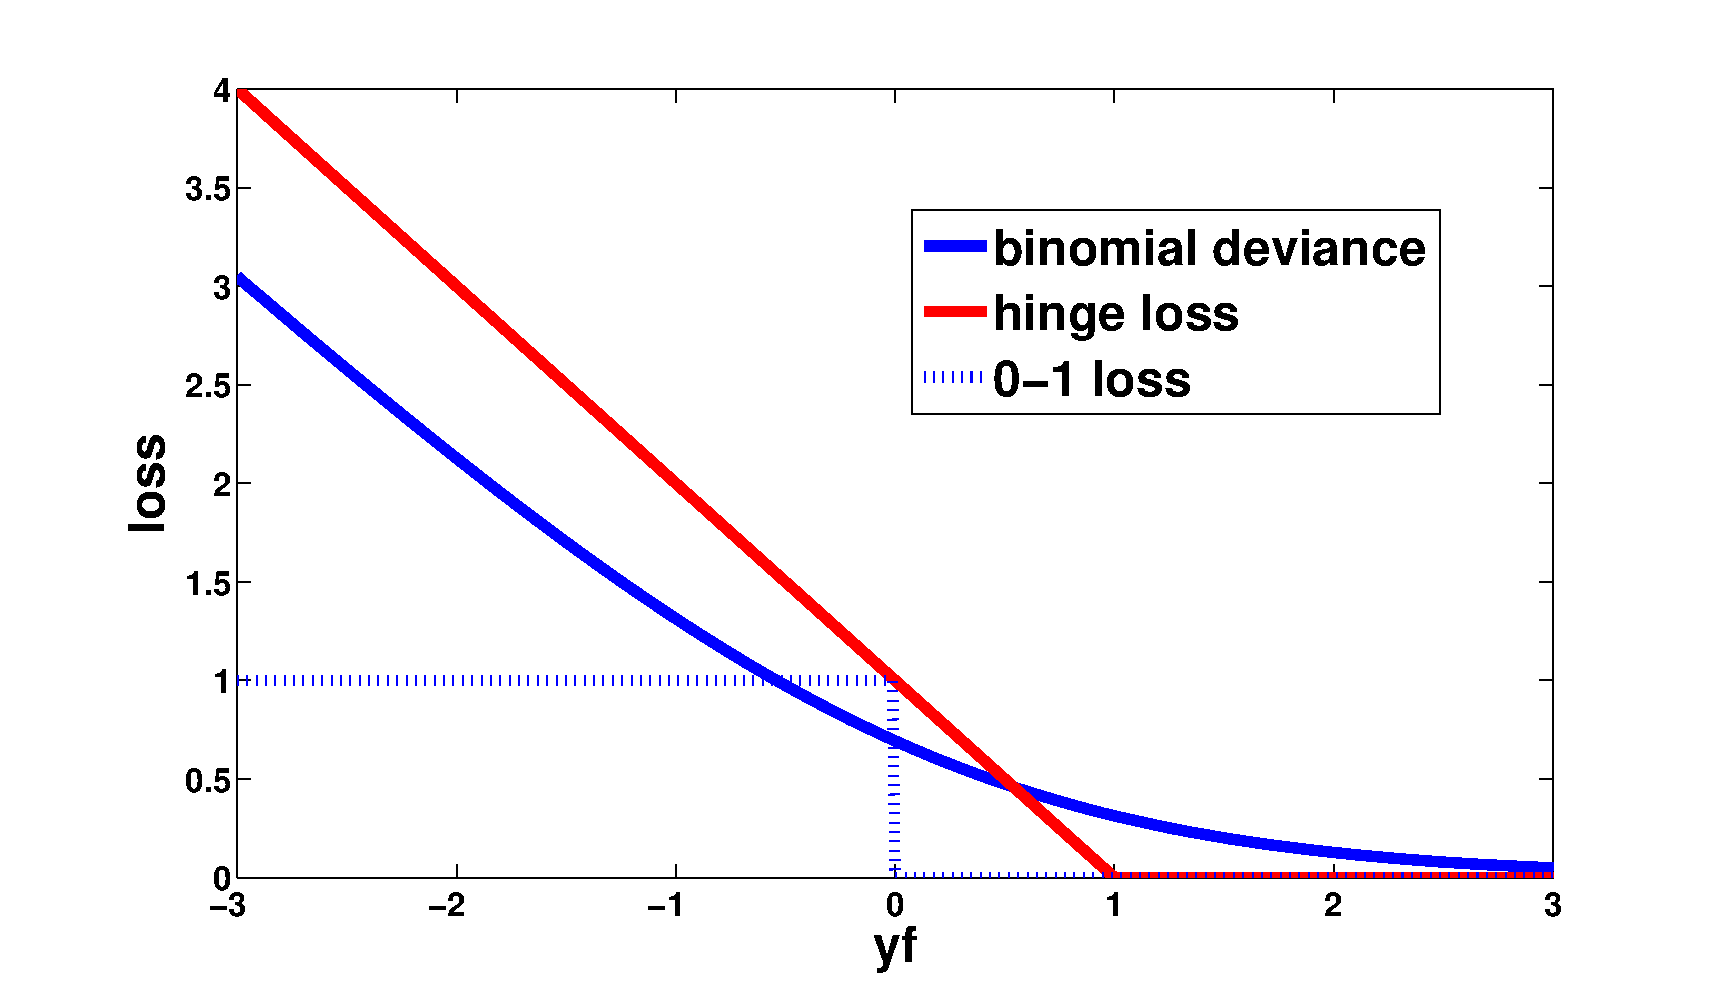
\includegraphics[width=0.6\textwidth]{lossclassification.eps}
  \end{center}
\end{figure}
\dis { What differences ?  Computational issues ? Which data examples
feel the ``gradient'' force?}
}


%%%%-------------------------------------------
\frame{


\begin{ex}
Consider the minimization problem 
\[ \inf_f \e \ell_{hinge} (Y, f(X))\]
for the $\set{\pm 1}$-encoded binary classification problem.
Show that the optimal $f^*_{hinge}$ is 
$\mbox{sign}(h(x)-0.5  )$
where $h(x)=\p(Y=+1\vert X=x)$.
\end{ex}
Recall a similar exercise for the binomial deviance loss.

\biz
\item
Note  $\mbox{sign}(f^*_{hinge})=f^*_{hinge}$ 
since $f^*_{hinge}$ only takes value $\pm 1$.
\item $f^*_{bd}$ is continuous, but $f^*_{hinge}$
is a step-type function.
\eiz
%\noindent\rule{\textwidth}{0.5pt}
}

\frame{

\footnotesize
\begin{align*}
  &\e \ell_{hinge} (Y, f(X))\\
=&
\pi_+ \e_{X|Y=+1} \ell_{hinge} (+1, f(X))   
+\pi_-\e_{X|Y=-1} \ell_{hinge} (+1, f(X)) 
\\
= &\pi_+  \int_\Xcal I(1-f(x)>0) \, (1-f(x))\,  \rho_+(x)\dx \\
& ~
+\pi_-  \int_\Xcal I(1+f(x)>0)\, (1+f(x)) \, \rho_-(x)\dx 
\end{align*}
Consider the domain $\Omega_+ \subset \Xcal $
where $f(x)>1$, then the integration over 
$\Omega_+$ is 
$\pi_-\int_{\Omega_+}  (1+f(x) )\rho_-(x) \dx$:
by decreasing the value of $f$ on this domain $\Omega_+$
to the minimal possible value $1$, one has a smaller loss.
So, for $f^*$ to be optimal, $\Omega_+$ must be empty.
For the same reason for $\Omega_-$ case, we deduce that 
$f^*(x) \in [-1,1]$ almost everywhere.
Then we only consider to minimize within  this bounded function class
$\set{f: \abs{f(x)} \leq 1}$
$\pi_+  \int_\Xcal  (1-f(x))\,  \rho_+(x)\dx
+\pi_-  \int_\Xcal   (1+f(x)) \, \rho_-(x)\dx 
= \int_{\Xcal} f(x)  \left ( \pi_-  \rho_-(x)  -\pi_+\rho_+(x) \right)  \dx
+ 1
$. So if $\pi_-\rho_-(x) <\pi_+\rho_+(x)$,
the minimizer is $f^*(x)=1$;
otherwise $f^*(x)=-1$. Equivalently,
$f^*(x)=\sign(\pi_+\rho_+(x) - \pi_+\rho_+(x) )
=\sign(h(x)-0.5)$
since $h(x)= \frac{\pi_+\rho_+(x)}{ 
\pi_+\rho_+(x) + \pi_+\rho_+(x) 
}
 $

}


%%%-------------------------------------

\frame{
{ Regularization  in SVM smoothes $f^*_{hinge}$}
\biz
\item
The  objective function with regularization 
$$\inf_{f\in \Hcal}  \e \ell_{hinge} (Y, f(X))  + \lambda R(f)$$ 
gives a smooth function approximation $f_\lambda$ to
the step function $f^*_{hinge}$, and the classifier is 
$$x\to \mbox{sign}(f_\lambda)$$
places back $f_\lambda$ to step function by thresholding. 
\item
For SVC, the hypothesis space $\Hcal$ is linear function space,
and SVC use  a linear function to approximate a step  function with jumps. The maximal margin $\|w\|$  has the meaning of penalty.
\eiz
}

\frame{{topics not touched here for SVM}
\biz
\item kernel trick, RKHS
\item optimization theory and methods for SVM
\eiz
}

\end{document}


